% Chapter 3

\chapter{METHODOLOGICAL FRAMEWORKS} % Main chapter title

\label{Chapter3} % Change X to a consecutive number; for referencing this chapter elsewhere, use \ref{ChapterX}

\lhead{Chapter 3. \emph{Methodological Frameworks}} % Change X to a consecutive number; this is for the header on each page - perhaps a shortened title

%----------------------------------------------------------------------------------------
%	SECTION 1
%----------------------------------------------------------------------------------------



%\begin{figure}[htbp]
%	\centering
%	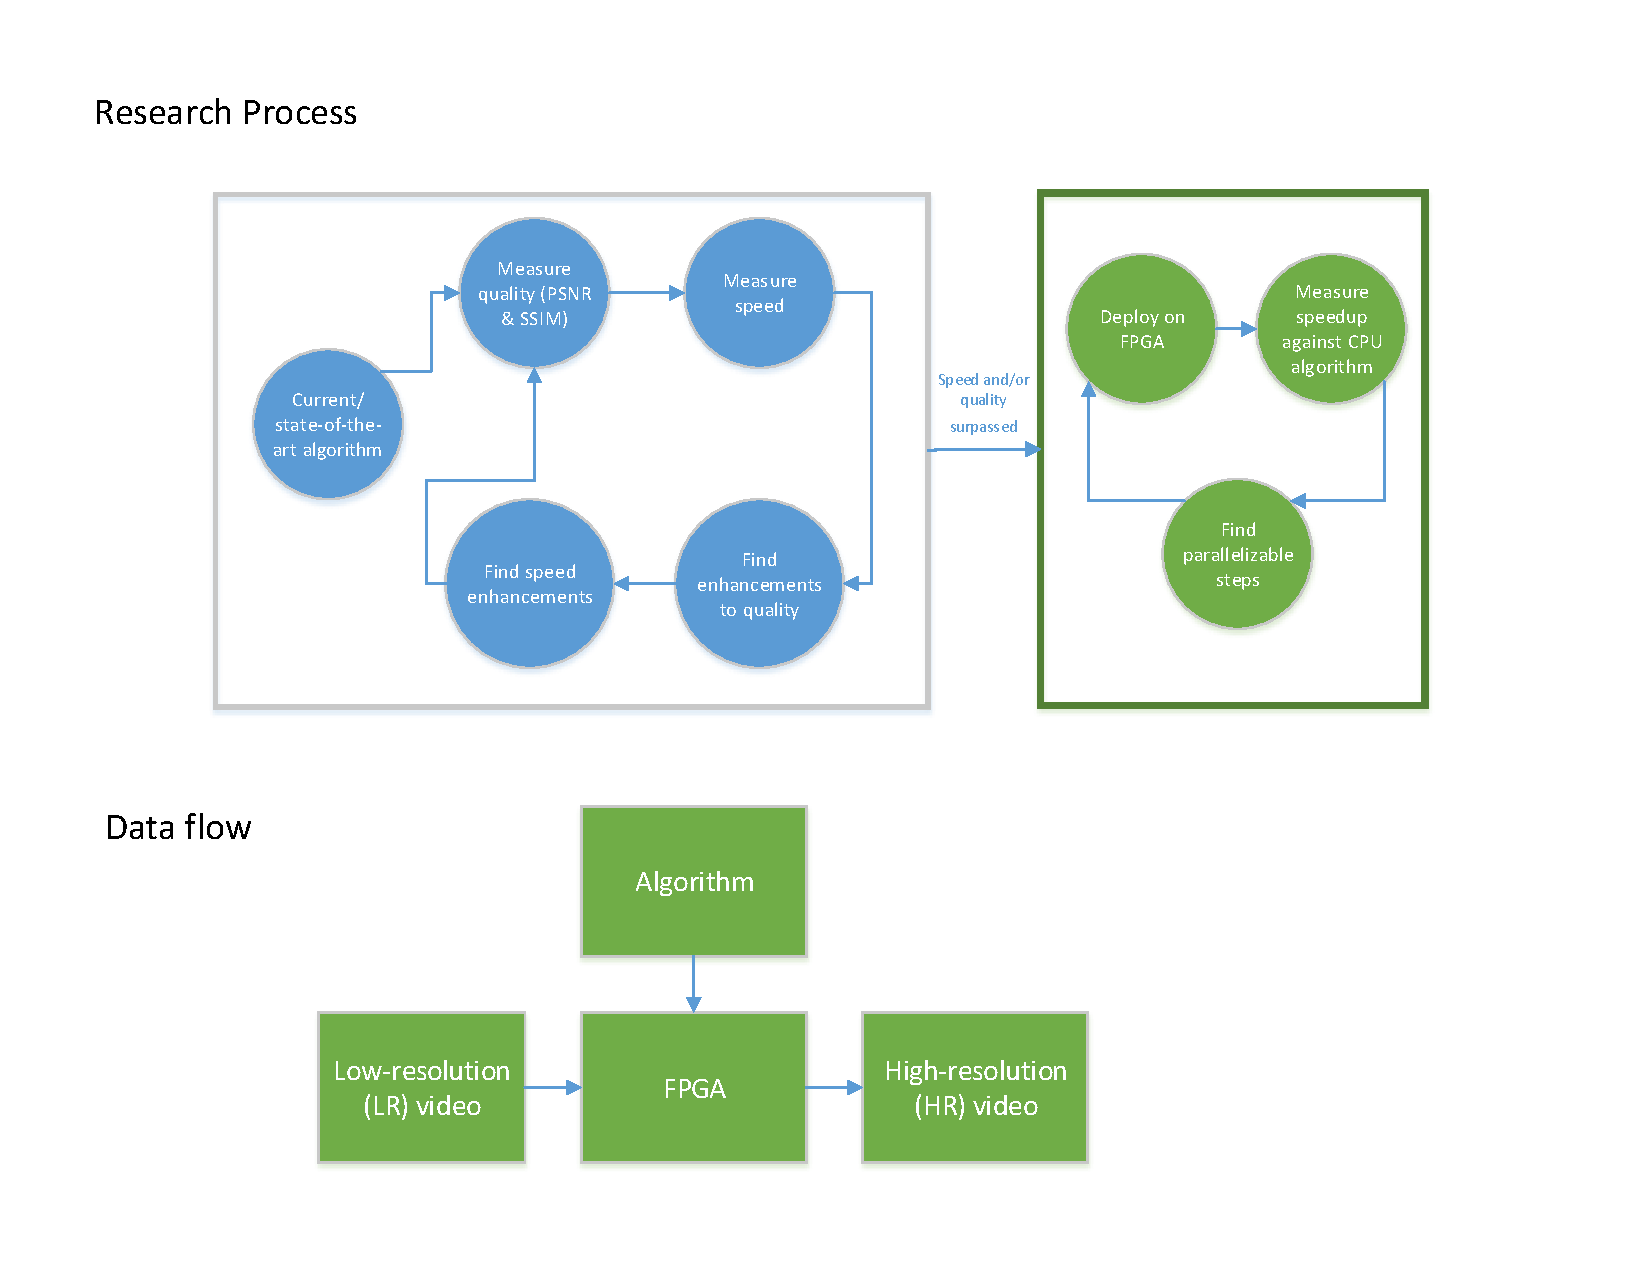
\includegraphics{Figures/framework.pdf}
%	\rule{35em}{0.2pt}
%	\caption[Conceptual Framework]{Conceptual Framework of the Study.}
%	\label{fig:Framework}
%\end{figure}



%-----------------------------------
%	SUBSECTION 1
%-----------------------------------
\section{Image Quality Assessment (IQA)}

For image quality to be assessed in the study, three metrics will be used.
They are the peak signal-to-noise ratio (PSNR), the structural similarity index measure (SSIM), and the feature similarity index measure (FSIM). The PSNR measures the robustness the algorithm against noise found in the LR image.
The SSIM measures how similar two images are to one another, ACCO

Given a reference image \textit{a} and a test image \textit{b}, both of the same size \textit{M}x\textit{N},the PSNR is computed using the following equation \citep{Hore2010}:

\begin{equation}
PSNR(a,b) = 20 \log_{10}\frac{255}{\sqrt{MSE(a,b)}}
\end{equation}

where the MSE (mean squared error) is computed as follows:
\begin{equation}
MSE(a,b) = \frac{1}{MN} \sum\limits_{i=1}^{M} \sum\limits_{j=1}^{N} (a_{ij}-b_{ij})^2
\end{equation}


The SSIM is computed using the following equation \citep{Hore2010}:

\begin{equation}
SSIM(a,b) = l(a,b) c(a,b) s(a,b)
\end{equation}

where
\begin{eqnarray}
l(a,b) = \frac{2\mu_a\mu_b+C_1}{\mu_a^2+\mu_b^2+C_1} \label{eqn:luminance_ssim}\\
c(a,b) = \frac{2\sigma_a\sigma_b+C_2}{\sigma_a^2+\sigma_b^2+C_2}\label{eqn:contrast_ssim}\\
s(a,b) = \frac{\sigma_{ab}+C_3}{\sigma_a\sigma_b+C_3}\label{eqn:structure_ssim}
\end{eqnarray}

Equation \ref{eqn:luminance_ssim} measures the similarity in luminance and is equal to 1 only if $\mu_a=\mu_b$.
Similarly, equation \ref{eqn:contrast_ssim} compares the standard deviation of the two images (which corresponds to the contrast). 
It will only equal to 1 if $\sigma_a=\sigma_b$.
The structure comparison equation (\ref{eqn:structure_ssim}) measures the correlation between the images using the covariance $\sigma_{ab}$ between them.

The FSIM is computed using the following equation \citep{Zhang2011a}:

\begin{equation}
\frac{\sum_{x\in\Omega}S_L(\mathbf{x})\cdot PC_m(\mathbf{x})}{{\sum_{x\in\Omega}PC_m(\mathbf{x})}}
\end{equation}

where $\Omega$ is the whole spatial image domain and $S_L$ is the SSIM.
$S_L(\mathbf{x})$

\section{Algorithm Framework}

% Explain the framework
Figure \ref{fig:algoframe} summarizes the flow of the proposed algorithm.
The major components of this algorithm are the deblurring module, the temporal consistency module, and the edge-preservation module.

The deblurring module removes image blur caused by motion and the camera sensor.
To accomplish the process of deblurring, a blur kernel is first estimated.
Motion blur is usually modeled as
\begin{equation}
	B = K * L + N	
\end{equation}
where $B$ is the blurred image, $K$ is the motion blur kernel, $N$ is unknown noise introduced during image acquisition, and $*$ is the convolution operator \citep{Cho2009}.

To be able to deconvolve the $K$ and $L$ terms, both of these terms must be optimized in an alternating fashion.
\begin{equation}
L' = \argmin_L{(||B-K*L||+\rho_L(L))}
\end{equation}
\begin{equation}
K' = \argmin_K{(||B-K*L||+\rho_K(K))}
\end{equation}

The $\argmin$ notation denotes an operation to minimize the variable subscripted in the $\argmin$ subject to the constraints stated inside the parentheses.
The symbols $||$ represent a norm, a function that assigns a strictly positive length to each vector in a vector space except the zero vector.
It is typical to use the 2-dimensional, or $L_2$, norm, as it is the intuitive notion of length in any n-dimensional space, and is computationally efficient.
The additive term at the end of the equations are regularization terms.
This is added to prevent overfitting of the data or to provide additional information to solve an ill-posed problem.

The temporal consistency module ensures that successive video frames are consistently super-resolved with respect to time. 
It uses the preceding HR frame to accomplish this task.
Temporal consistency is computed as follows:

\begin{equation}
	C_t = exp(-\frac{1}{2\rho_0^2}||M_t^{t-1}X_t-\widetilde{X}_{t-1}||^2)
\end{equation}

where $X_t$ is the low-resolution frame at time $t$, $\widetilde{X}_{t-1}$ is the preceding high-resolution frame, $M_t$ is the motion matrix, and
\begin{equation}
\rho_0^2 = \rho \cdot var(B(\widetilde{M}_t^{t-1}\bar{X}_t-\widetilde{X}_{t-1} = 1))
\end{equation}
is the $l_0$ norm of the difference between the motion-blurred current frame and the previous high-resolution frame.

The edge-preservation module takes the finer details of the LR video frames and interpolates the HR version of the edges. 
This will be accomplished through weighted least-squares filtering \citep{Farbman2008}.

Given an image $g$ , we are attempting to find $u$ such that $u$ is as close as possible to $g$ while being smooth as possible everywhere, except across significant gradients in $g$. 
This is formalized as minimizing the equation

\begin{equation}
	(u-g)^T(u-g)+\lambda(u^T D_x^T A_x D_x u + u^T D_y^T A_y D_y u)
\end{equation}

where $A_x$ and $A_y$ are diagonal matrices containing the smoothness weights, and the matrices $D_x$ and $D_y$ are discrete differentiation operators.

A final reconstruction step incorporates output from all the three major modules to generate the HR frame sequence.

The three modules were built in parallel to each other so that the algorithm would be amenable to optimization on the FPGA side of the SoC.

% Place figure here
\begin{figure}[!ht]
	\centering
	\includegraphics[scale=0.7]{Figures/ALGO_FRAMEWORK.png}
	\caption[]{Framework for the Proposed Algorithm.}
	\label{fig:algoframe}
\end{figure}


%-----------------------------------
%	SUBSECTION 2
%-----------------------------------


\section{Hardware Framework}
Figure \ref{fig:hardframe} illustrates the flow of data across the hardware devices to be used in the study.
A video source such as a camera or prerecorded file will be sent for super-resolution on the SoC, which will then display the result on the monitor in real-time.
Initially a conventional computer will serve as the development and evaluation  environment for the SR algorithm.
This computer contains the MATLAB and Vivado software packages that are used for the development and testing of the algorithm in both the computer and the FPGA-CPU hybrid.
A version of the algorithm can then be sent to the SoC for testing and fine-tuning.

\begin{figure}[!ht]
	\centering
	\includegraphics[scale=0.7]{Figures/HARDWARE_FRAMEWORK.png}
	\caption[]{Framework for Hardware Implementation.}
	\label{fig:hardframe}
\end{figure}


% Explain the framework



%----------------------------------------------------------------------------------------
%	SECTION 2
%----------------------------------------------------------------------------------------
